\documentclass{article}
\usepackage[spanish]{babel}
\usepackage[utf8]{inputenc}
\usepackage{amsmath}
\usepackage{amssymb}
\usepackage{amsthm}
\usepackage{graphics}
\usepackage{subfigure}
\usepackage{lipsum}
\usepackage[mathscr]{euscript}
\usepackage{array}
\usepackage{multicol}
\usepackage{enumerate}
\usepackage[framemethod=TikZ]{mdframed}
\usepackage[a4paper, margin = 1.5cm]{geometry}
\usepackage{fullpage}

%En esta parte se hacen redefiniciones de algunos comandos para que resulte agradable el verlos%

\renewcommand{\theenumii}{\roman{enumii}}

\def\proof{\paragraph{Demostración:\\}}
\def\endproof{\hfill$\blacksquare$\\}

\def\sol{\paragraph{Solución:\\}}
\def\endsol{\hfill$\square$\\}

%En esta parte se definen los comandos a usar dentro del documento para enlistar%

\newtheoremstyle{largebreak}
  {}% use the default space above
  {}% use the default space below
  {\normalfont}% body font
  {}% indent (0pt)
  {\bfseries}% header font
  {}% punctuation
  {\newline}% break after header
  {}% header spec

\theoremstyle{largebreak}

\newmdtheoremenv[
    leftmargin=0em,
    rightmargin=0em,
    innertopmargin=-2pt,
    innerbottommargin=8pt,
    hidealllines = true,
    roundcorner = 5pt,
    backgroundcolor = gray!60!red!30
]{exa}{Ejemplo}[section]

\newmdtheoremenv[
    leftmargin=0em,
    rightmargin=0em,
    innertopmargin=-2pt,
    innerbottommargin=8pt,
    hidealllines = true,
    roundcorner = 5pt,
    backgroundcolor = gray!50!blue!30
]{obs}{Observación}[section]

\newmdtheoremenv[
    leftmargin=0em,
    rightmargin=0em,
    innertopmargin=-2pt,
    innerbottommargin=8pt,
    rightline = false,
    leftline = false
]{theor}{Teorema}[section]

\newmdtheoremenv[
    leftmargin=0em,
    rightmargin=0em,
    innertopmargin=-2pt,
    innerbottommargin=8pt,
    rightline = false,
    leftline = false
]{propo}{Proposición}[section]

\newmdtheoremenv[
    leftmargin=0em,
    rightmargin=0em,
    innertopmargin=-2pt,
    innerbottommargin=8pt,
    rightline = false,
    leftline = false
]{cor}{Corolario}[section]

\newmdtheoremenv[
    leftmargin=0em,
    rightmargin=0em,
    innertopmargin=-2pt,
    innerbottommargin=8pt,
    rightline = false,
    leftline = false
]{lema}{Lema}[section]

\newmdtheoremenv[
    leftmargin=0em,
    rightmargin=0em,
    innertopmargin=-2pt,
    innerbottommargin=8pt,
    roundcorner=5pt,
    backgroundcolor = gray!30,
    hidealllines = true
]{mydef}{Definición}[section]

\newmdtheoremenv[
    leftmargin=0em,
    rightmargin=0em,
    innertopmargin=-2pt,
    innerbottommargin=8pt,
    roundcorner=5pt
]{excer}{Ejercicio}[section]

%En esta parte se colocan comandos que definen la forma en la que se van a escribir ciertas funciones%
\newcommand{\norm}[1]{\ensuremath{\|#1\|}}
\newcommand\subtitle[1]{\textit{\large #1}\\}
\newcommand\abs[1]{\ensuremath{\left|#1\right|}}
\newcommand\divides{\ensuremath{\bigm|}}
\newcommand\cf[3]{\ensuremath{#1:#2\rightarrow#3}}
\newcommand\natint[1]{\ensuremath{\left[\!\left[ #1\right]\!\right]}}
\newcommand{\afa}{\:
    \begin{tikzpicture}
        \draw [line width = 0.17 mm, black] (0,0) -- (-0.115,0.29);
        \draw [line width = 0.17 mm, black] (0,0) -- (0.115,0.29);
        \draw [line width = 0.17 mm, black] (-0.12,0) arc (190:-10:0.12cm);
    \end{tikzpicture}
    \:
}
%Este símvolo es para casi todo salvo una cantidad finita

%recuerda usar \clearpage para hacer un salto de página

\begin{document}

    \title{Taller Topología Algebraica, Lectura 2: El Grupo Fundamental}
    \author{Cristo Alvarado}
    \setcounter{section}{2}
    \maketitle

    \subtitle{Grupo Fundamental}

    Como resultado de este lema, se puede definir la multiplicación de clases de equivalencia de caminos (de tal suerte que el punto terminal del primer camino coincida con el inicial del segundo camino).
    
    \begin{mydef}
        Sea $X$ espacio y $f,g$ caminos en $X$ tales que el punto terminal de $f$ es el punto inicial de $g$. $\left[f\right]$ denota a la \textbf{clase de equivalencia con representante $f$} y $\left[g\right]$ a la de $g$.

        Se define el producto de las clases $[f]$ y $[g]$ por:
        \begin{equation*}
            [f]\cdot[g]=[f\cdot g]
        \end{equation*}
    \end{mydef}

    Debido al lema anterior, el producto de clases de equivalencia está bien definido.

    Este es el tipo de multiplicación que nos va a concerner en lo que sigue. En general, la multiplicación de caminos no es asociativa.

    \begin{excer}[\textbf{La multiplicación de caminos no es asociativa.}]
        Considere en $\mathbb{R}^3$ dotado de la topología usual los caminos
        \begin{equation*}
            f(t)=(t,0,0),\quad g(t)=(0,t,0)\quad\textup{y}\quad h(t)=(0,0,t)
        \end{equation*}
        para todo $t\in I$. Compute $f\cdot (g\cdot h)$ y $(f\cdot g)\cdot h$.
    \end{excer}

    Sin embargo, se tiene el siguiente resultado:

    \begin{lema}
        La multiplicación de clases de equivalencia de caminos es asociativa.
    \end{lema}

    \begin{proof}
        Sean $f,g,h$ caminos en $X$ tales que el punto terminal de $f$ es el punto inicial de $g$ y el punto terminal de $g$ es el punto inicial de $h$. Se tiene entonces que los productos:
        \begin{equation*}
            f\cdot (g\cdot h)\quad\textup{y}\quad (f\cdot g)\cdot h
        \end{equation*}
        están bien definidos (\textit{verificar!}). Para probar el resultado, debemos ver que
        \begin{equation*}
            [f]\cdot \left([g]\cdot [h]\right)=\left([f]\cdot[g] \right)\cdot [h]
        \end{equation*}
        lo que es equivalente a probar que
        
        \begin{equation*}
            [f\cdot (g\cdot h)]=[(f\cdot g)\cdot h]
        \end{equation*}
        es decir, que $f\cdot (g\cdot h)\sim(f\cdot g)\cdot h$. Considere la función $\cf{F}{I\times I}{X}$ dada por:
        \begin{equation*}
            F(t,s)=\left\{
                \begin{array}{lcr}
                    f\left(\frac{4t}{1+s}\right) & \textup{ si } & 0\leq t\leq\frac{s+1}{4}\\
                    g(4t-1-s) & \textup{ si } & \frac{s+1}{4}\leq t\leq\frac{s+2}{4}\\
                    h\left(1-\frac{4(1-t)}{2-s}\right) & \textup{ si } & \frac{s+2}{4}\leq t\leq 1\\
                \end{array}
            \right.
        \end{equation*}

        \begin{figure}
            \begin{center}
                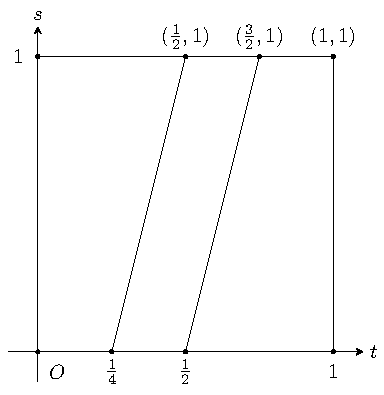
\includegraphics[scale=1]{images/fig_1.pdf}
            \end{center}
            \caption{Dominio de la función $F$.}
        \end{figure}

        para todo $s,t\in I$. Queda como ejercicio probar que $F$ es continua.
    \end{proof}

    Para cualquier punto $x\in X$, denotemos por $\mathscr{I}_x=[i_x]$ a la clase de equivalencia del mapeo identidad, es decir $\cf{i_x}{I}{X}$ es tal que $i_x(t)=x$ para todo $y\in I$. Esta clase tiene la siguiente propiedad fundamental:

    \begin{lema}
        Sea $\mathscr{F}=[f]$ una clase de equivalencia de caminos con punto inicial $x\in X$ y terminal $y\in X$. Entonces, $\mathscr{I}_x\cdot\mathscr{F}=\mathscr{F}$ y $\mathscr{F}\cdot\mathscr{I}_y=\mathscr{F}$.
    \end{lema}

    \begin{proof}
        Solo se probará la primera igualdad, para ello, basta con probar que $i_x\cdot f\sim f$. En efecto, defina la función $\cf{F}{I\times I}{X}$ dada por:
        \begin{equation*}
            F(t,s)=\left\{
                \begin{array}{lcr}
                    x & \textup{ si } & 0\leq t\leq\frac{s}{2}\\
                    f\left(\frac{2t-s}{2-s}\right) & \textup{ si } & \frac{s}{2}\leq t\leq 1\\
                \end{array}
            \right.
        \end{equation*}
        para todo $s,t\in I$. Entonces, $F(t,0)=f(t)$ y $F(t,1)=(e\cdot f)(1)$ siendo $F$ continua. Por tanto, $\mathscr{I}_x\cdot\mathscr{F}=\mathscr{F}$.
    \end{proof}

    En cierto modo, lo que decimos es que la clase $\mathscr{I}_x$ actúa como elemento identidad (\textit{¿De dónde?}).

    \begin{mydef}
        Para cualquier camino $\cf{f}{I}{X}$, $\overline{f}$ denota al camino definido por:
        \begin{equation*}
            \overline{f}(t)=f(1-t),\quad\forall t\in I
        \end{equation*}
        El camino $\overline{f}$ se obtiene recorriendo el camino $f$ en sentido contrario.
    \end{mydef}

    \begin{lema}
        Sea $f$ un camino y denotemos por $\mathscr{F}=[f]$ y $\overline{\mathscr{F}}=[\overline{f}]$, entonces:
        \begin{equation*}
            \mathscr{F}\cdot\overline{\mathscr{F}}=\mathscr{I}_x\quad\textup{y}\quad\overline{\mathscr{F}}\cdot\mathscr{F}=\mathscr{I}_y
        \end{equation*}
        donde $x\in X$ y $y\in X$ son los puntos inicial y terminal de $f$, respectivamnete.
    \end{lema}

    \begin{proof}
        Sólo se probará la primera igualdad, para ello es suficiente con probar que $f\cdot\overline{f}\sim i_x$. Definimos la función $\cf{F}{I\times I}{X}$ por:
        \begin{equation*}
            F(t,s)=\left\{
                \begin{array}{lcr}
                    f(2t) & \textup{ si } & 0\leq t\leq\frac{s}{2}\\
                    f(s) & \textup{ si } & \frac{s}{2}\leq t\leq1-\frac{s}{2}\\
                    f(2-2t) & \textup{ si } & 1-\frac{s}{2}\leq t\leq1\\
                \end{array}
            \right.
        \end{equation*}
        para todo $s,t\in I$. Entonces,
        \begin{equation*}
            \begin{split}
                F(t,0)&=\left\{
                    \begin{array}{lcr}
                        f(2t) & \textup{ si } & 0\leq t\leq0\\
                        f(s) & \textup{ si } & 0\leq t\leq1-0\\
                        f(2-2t) & \textup{ si } & 1-0\leq t\leq1\\
                    \end{array}
                \right.\\
                &=\left\{
                    \begin{array}{lcr}
                        f(0) & \textup{ si } & t=0\\
                        f(0) & \textup{ si } & 0\leq t\leq1\\
                        f(2-2t) & \textup{ si } & t=1\\
                    \end{array}
                \right.\\
                &=\left\{
                    \begin{array}{lcr}
                        x & \textup{ si } & 0\leq t\leq1\\
                        f(0) & \textup{ si } & t=1\\
                    \end{array}
                \right.\\
                &=x\\
            \end{split}
        \end{equation*}
        para todo $t\in I$. Además,
        \begin{equation*}
            \begin{split}
                F(t,1)&=\left\{
                    \begin{array}{lcr}
                        f(2t) & \textup{ si } & 0\leq t\leq\frac{1}{2}\\
                        f(1) & \textup{ si } & \frac{1}{2}\leq t\leq1-\frac{1}{2}\\
                        f(2-2t) & \textup{ si } & 1-\frac{1}{2}\leq t\leq1\\
                    \end{array}
                \right.\\
                &=\left\{
                    \begin{array}{lcr}
                        f(2t) & \textup{ si } & 0\leq t\leq\frac{1}{2}\\
                        f(1-(2t-1)) & \textup{ si } & \frac{1}{2}\leq t\leq1\\
                    \end{array}
                \right.\\
                &=\left\{
                    \begin{array}{lcr}
                        f(2t) & \textup{ si } & 0\leq t\leq\frac{1}{2}\\
                        \overline{f}(2t-1) & \textup{ si } & \frac{1}{2}\leq t\leq1\\
                    \end{array}
                \right.\\
                &=f\cdot\overline{f}(t)\\
            \end{split}
        \end{equation*}
        para todo $t\in I$. Queda como ejercicio probar que la función $F$ es continua.

        Por tanto, $\mathscr{F}\cdot\overline{\mathscr{F}}$.
    \end{proof}

    En visata de estas propiedades de la clase $\overline{\mathscr{F}}$, de ahora en adelante la denotaremos por $\mathscr{F}^{-1}$.

    Podemos resumir todos los lemas antes probados diciendo que el conjunto de todas las clases de caminos en un espacio $X$ satisfacen los axiomas de grupo, excepto que el producto de dos caminos no siempre está definido. Solventamos este problema con la siguiente definición:

    \begin{mydef}
        Un camino o una clase de camino es llamada \textbf{cerrada} o un \textbf{bucle}, si el punto inicial y terminal son el mimso. El bucle se dice que tiene \textbf{base} en el punto inicial o terminal.
    \end{mydef}

    \begin{theor}
        Sea $X$ un espacio topológico y $x\in X$ un punto fijo. Entonces, el conjunto de todas las clases de caminos cerradas que tienen como punto base a $x$ dotado por la operación $\cdot$, denotado por $\pi(X,x)$ es un grupo llamado \textbf{grupo fundamental} o \textbf{grupo de Poincaré} de $X$ con punto base $x$.
    \end{theor}

    \begin{proof}
        Es un resumen de todos los lemas anteriores.
    \end{proof}
    
    \begin{obs}
        Para un espacio topológico dado $X$ y $x\in X$, dotamos el grupo fundamental $\pi(X,x)$ de una operación binaria que lo hace de grupo, de ahora en adelante tal operación se denotará al producto de dos clases $[f]$ y $[g]$ por $[f]\cdot[g]$ o por yuxtaposición como $[f][g]=[f\cdot g]$ (no confundir la operación dentro de los paréntesis cuadrados con la composición usual de funciones).

        Si $[f]\in\pi(X,x)$, se denotará a su inverso por $[f]^{-1}$ y, al elemento identidad por $\mathscr{I}$
    \end{obs}

    \begin{propo}
        Sea $X$ un espacio y $x,y\in X$ dos puntos distintos. Si $\cf{\gamma}{I}{X}$ es un camino con punto inicial $x$ y terminal $y$, entonces $\pi(X,x)\cong\pi(X,y)$ (es decir, son grupos isomorfos).
    \end{propo}

    \begin{proof}
        En efecto, defina la función $\cf{u}{\pi(X,x)}{\pi(X,y)}$ dada por:
        \begin{equation*}
            u([f])=[\gamma]^{-1}[f][\gamma]
        \end{equation*}
        Por cursos anteriores de teoría de Grupos, se ve de forma inmediata que esta función es un isomorfismo entre los grupos $\pi(X,x)$ y $\pi(X,y)$.
    \end{proof}

    \begin{cor}
        Sea $X$ un espacio topológico arco-conexo, entonces los grupos $\pi(X,x)$ y $\pi(X,y)$ son isomorfos para todo $x,y\in X$.
    \end{cor}

    La importancia del teorema anterior radica en que el grupo $\pi(X,x)$ tiene propiedades como grupo (es decir, es abeliano, finito, nilpotente, libre, etc...) no debido al punto elegido $x\in X$, sino al espacio mismo $X$, suponiendo que $X$ es arco-conexo.

    En general, no hay un mapeo canónico o isomorfismo natural entre $\pi(X,x)$ y $\pi(X,y)$, ya que a cada elección de camino entre $x$ y $y$ le corresponderá un isomorfismo.\\

    \subtitle{Efecto de una función continua en el grupo fundamental}

    \begin{obs}
        Para esta sección resultará de utilidad definir el siguiente conjunto, para todo espacio topológico $X$ se define
        \begin{equation*}
            \wp_X = \bigcup \left\{[f]\Big|\cf{f}{I}{X}\textup{ es una función continua} \right\}
        \end{equation*}
        es decir, estamos tomando todas las clases de caminos de un espacio topológico $X$ (note que no tiene nada que ver con el grupo fundamental, más que con el hecho de que usa las clases de caminos en su definición).
    \end{obs}

    Considere dos espacios topológicos $X$ y $Y$ y sea $\cf{\varphi}{X}{Y}$ una función continua. Si $\cf{f_0,f_1}{I}{X}$ son caminos en $X$, ¿también lo son $\varphi\circ f_0$ y $\varphi\circ f_1$?

    \begin{propo}
        Sean $X$ y $Y$ espacios topológicos, $\cf{f_0,f_1}{I}{X}$ caminos equivalentes. Entonces, $\varphi\circ f_0\sim \varphi\circ f_1$.
    \end{propo}

    \begin{proof}
        Como $f_1\sim f_0$, existe pues una función continua $\cf{F}{I\times I}{X}$ tal que
        \begin{equation*}
            F(x,0)=f_0(x),\quad F(x,1)=f_1(x)
        \end{equation*}
        para todo $x\in I$ y,
        \begin{equation*}
            F(0,t)=f_0(0)=f_1(0),\quad F(1,t)=f_0(1)=f_1(1)
        \end{equation*}
        Considere la función $\cf{G}{I\times I}{Y}$ dada por:
        \begin{equation*}
            G(x,t)=\varphi\circ F(x,t)
        \end{equation*}
        Es claro que esta funciónes continua por ser composición de funciones continuas, además se cumple que
        \begin{equation*}
            \begin{split}
                G(x,0)&=\varphi\circ F(x,0)\\
                &=\varphi (F(x,0))\\
                &=\varphi (f_0(x))\\
                &=\varphi\circ f_0(x)\\
            \end{split}
        \end{equation*}
        para todo $x\in I$. De forma análoga
        \begin{equation*}
            G(x,1)=\varphi\circ f_1(x)
        \end{equation*}
        La otra condición se verifica de forma inmediata, con lo que se concluye que $\varphi\circ f_0\sim \varphi\circ f_1$.
    \end{proof}

    Con la proposición anterior, podemos definir sin problemas una función que mapee clases de caminos en $X$ a clases de caminos en $Y$, a partir de la función continua $\varphi$. Esto se hará con el objetivo de ver qué sucede con el grupo fundamental bajo esta función continua $\varphi_*$.

    \begin{mydef}
        Sean $X$ y $Y$ espacios topológicos y $\cf{\varphi}{X}{Y}$ una función continua. Sea $\cf{f}{I}{X}$ un camino que une a los puntos $x,y\in X$, se define la función $\cf{\varphi_*}{\wp_X}{\wp_Y}$ por
        \begin{equation*}
            \varphi_*([f])=[\varphi\circ f]
        \end{equation*}
        por la proposición anterior, esta función está bien definida.
    \end{mydef}

\end{document}